% !TEX TS-program = pdflatex
% !TEX encoding = UTF-8 Unicode
% !TEX root = ../ArsClassica.tex

%************************************************
\chapter{L'opera Sp.I.R.E}
\label{chp:L'opera Sp.I.R.E}
%************************************************

\epigraph{[...] bello come la retrattilità degli artigli degli uccelli rapaci; o ancora, come l'incertezza dei movimenti muscolari nelle pieghe delle parti molli della regione cervicale posteriore; [...] e soprattutto, come l'incontro fortuito su un tavolo di dissezione di una macchina da cucire e di un ombrello!}{Isidore Lucien Ducasse \\}

Tutto ebbe inizio nel luglio del 2017. \\
Nel corso della manifestazione \textit{ArteScienza} al Goethe Institute venne invitato il compositore francese, Pierre Jodlowski. In scena, il suo lavoro compositivo \textit{Ombra della Mente} ispirato ad alcuni scritti di Alda Merini. \\
Il lavoro di Jodlowski era basato su una parte teatrale recitata e una parte musicale, eseguita da una clarinettista e da una soprano (la voce recitante). La fusione tra momenti prettamente teatrali e parti musicali ebbero un effetto tagliente sulla mia produzione musicale. Ogni intervento recitante era contrappuntato da rumori prodotti tramite lo strofinio di una matita su un foglio di carta e la frizione di una piccola molla presente nella meccanica della lampada di scena. Il tutto era elaborato in live electronics. L'effetto della molla sfregata, amplificata da un microfono a contatto, mi ha fatto riaffiorare alla mente molti concerti di musica underground seguiti in passato (l'utilizzo delle molle, oltre ad appartenere all'universo della musica colta è stato abusato in ambienti musicali \textit{noise}\footnote{genere che utilizza il rumore come base principale per creare delle composizioni \\} e di musica cosiddetta "industriale" proprio per sottolineare l'utilizzo di materiale di scarto di industrie e fabbriche).
\begin{quotation}
Il paesaggio sonoro \textit{lo-fi} nasce dalla congestione sonora\footnote{R. Murray Schafer, \textit{Il paesaggio sonoro}, Casa Ricordi s.r.l. e LIM edizioni, 1985 \\}.
\end{quotation}
Andando avanti negli studi ho notato, poi, che già negli anni '50 del Novecento, John Cage cercò di far percepire, tramite l'amplificazione di elettromagneti e microfoni, i suoni non udibili. Durante il corso di \textit{interpretazione del partitura elettroacustica} del M° Giuseppe Silvi abbiamo ripercorso tutto lo scenario cagiano e da lì, ho iniziato ad interessarmi in modo più serio all'universo delle molle e alle loro particolarità timbriche. 
\begin{small}
\begin{quotation}
Si può dire che la musica moderna in generale è stata la storia della liberazione della dissonanza, così la nuova musica è parte del tentativo di liberare tutti i suoni udibili dalle limitazioni del pregiudizio musicale.
Un singolo suono in sé non è né musicale né non musicale; è semplicemente suono. [...] \\
La musica mi sembrava ora l'organizzazione del suono, l'organizzazione di qualunque suono ottenuto con qualunque mezzo\footnote{John Cage, \textit{Confessioni di un compositore} in AA.VV. (a cura di G. Bonomo e G. Furghieri), \textit{Riga n° 15} - John Cage, Milano, Marcos y Marcos, Milano 1998 \\}.
\end{quotation}
\end{small}
Le ricerche continuarono. Fortuito fu il lavoro fatto assieme al M° Michelangelo Lupone al Centro di Ricerche Musicali (CRM) sito in Roma. \\
Aiutai il maestro alla creazione di una sua installazione nell'estate del 2017. L'opera installativa, prodotta dall'artista Licia Galizia, era la scenografia interattiva della spettacolo coreutico \textit{Corpus 2.0}. Con il maestro, montammo sulla struttura della Galizia vari diffusioni e vari piezoelettrici che sarebbero poi serviti rispettivamente per la diffusione sonora e l'interazione con i danzatori. L'utilizzo dei diffusori applicati all'interno delle varie strutture e i trasduttori piezoelettrici che fungevano da parametri di controllo, mi hanno avvicinato ad un mondo a me limitrofo e ancora in parte sconosciuto. \\

\section{Necessità di uno strumento dedicato}
\addcontentsline{toc}{section}{Necessità di uno strumento dedicato}
\begin{small}
\begin{quotation}
Lo strumento musicale è il risultato di un insieme complesso di condizioni culturali. \\
Le sue caratteristiche tecnologiche e la sua \textit{structura} di oggeto composto devono consentire la rappresentazione di un determinato linguaggio musicale, caratterizzato da aspetti estetici, espressivi e stilistici che implicano una prassi esecutiva consolidata, o almeno condivisa in un determinato contesto\footnote{Silvia Lanzalone Strumenti aumentati in Acustica UTET}.
\end{quotation}
\end{small}
La creazione di uno strumento musicale, quindi, comporta molte problematiche sopratutto a livello stilistico e di concetto. La linea di confine tra uno strumento musicale e un oggetto che produce suono è strettamente legata al suo utilizzo. 
\begin{small}
\begin{quotation}
La ricerca di una definizione ontologica della musica è quindi strettamente connessa alla definizione dei confini tra un semplice oggetto che produce suono e uno strumento musicale, la cui prerogativa non può prescindere dal riconoscimento di un suo ruolo funzionale o simbolico in una data società
\footnote{\textit{ibidem}}.
\end{quotation}
\end{small}

Le giornate di lavoro al CRM diventavano fonte di suggestioni sull'utilizzo di oggetti risonanti e le loro capacità timbriche. Ogni oggetto sonoro diventava frutto di studio, anche minimo a volte, per via dei tempi brevi dati dalle consegne. Comunque, era un universo sonoro al quale aggrapparsi. \\
Giorno per giorno si andava a materializzare un'idea sempre più nitida, fino al giorno del mio esame del III anno di composizione elettroacustica. \\
Un esercizio, un brano, un piccolo studio sulle armoniche del pianoforte. La composizione partiva dalla trasformazione di un gesto sonoro: il pedale di risonanza in \textit{\textbf{fff}} seguito da cellule sonore inarmoniche composte da cluster e piccole volatine. I Gesti venivano elaborate tramite tre convoluzioni. Ogni convolutore apparteneva ad un universo sonoro a sé:
\begin{itemize}
\item{la prima convoluzione era la stessa cassa di risonanza del pianoforte eccitata dal pedale di risonanza calcato in \textit{\textbf{fff}};}
\item{la seconda convoluzione era creata registrando la molla della stessa lampada da tavolo utilizzata da Pierre Jodlowski nel suo lavoro;}
\item{la terza convoluzione era un'eccitazione del manico di una chitarra elettrica su un amplificatore a transistor.}
\end{itemize}

\begin{floatingfigure}{10cm}
\mbox{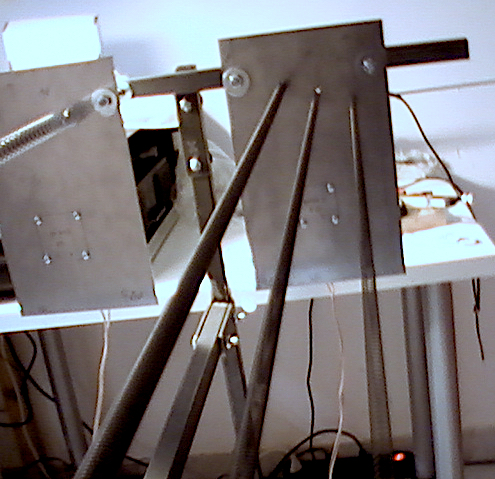
\epsfig{file=Prototipo01.jpg,width=8cm}}
\small{\caption{\textit{particolare}}}
\end{floatingfigure}
Ogni convoluzione era quindi legata ad un gesto, ma la cosa non mi soddisfaceva. Era come se volessi creare un convolutore che potesse essere, in qualche modo, anche un gesto scenico. Da qui alla creazione del mio iper-strumento, il passo è breve. Riuscii finalmente ad avere del tempo per finire di progettare il basamento, che prontamente un mio collega: Leonardo Mammozzetti, provvedette a costruire e a saldare. Piano piano l'oggetto prendeva forma, il CRM mi fornì le lastre mancanti e un mollificio, \textit{il mollificio Ciullo}, mi indirizzò nella scelta delle molle. Potei finalmente vedere, ma soprattutto sentire, se tutte le mie idee portavano a qualcosa di reale. \\
Era nato lo Sp.I.R.E. \\
\begin{floatingfigure}{10cm}
\mbox{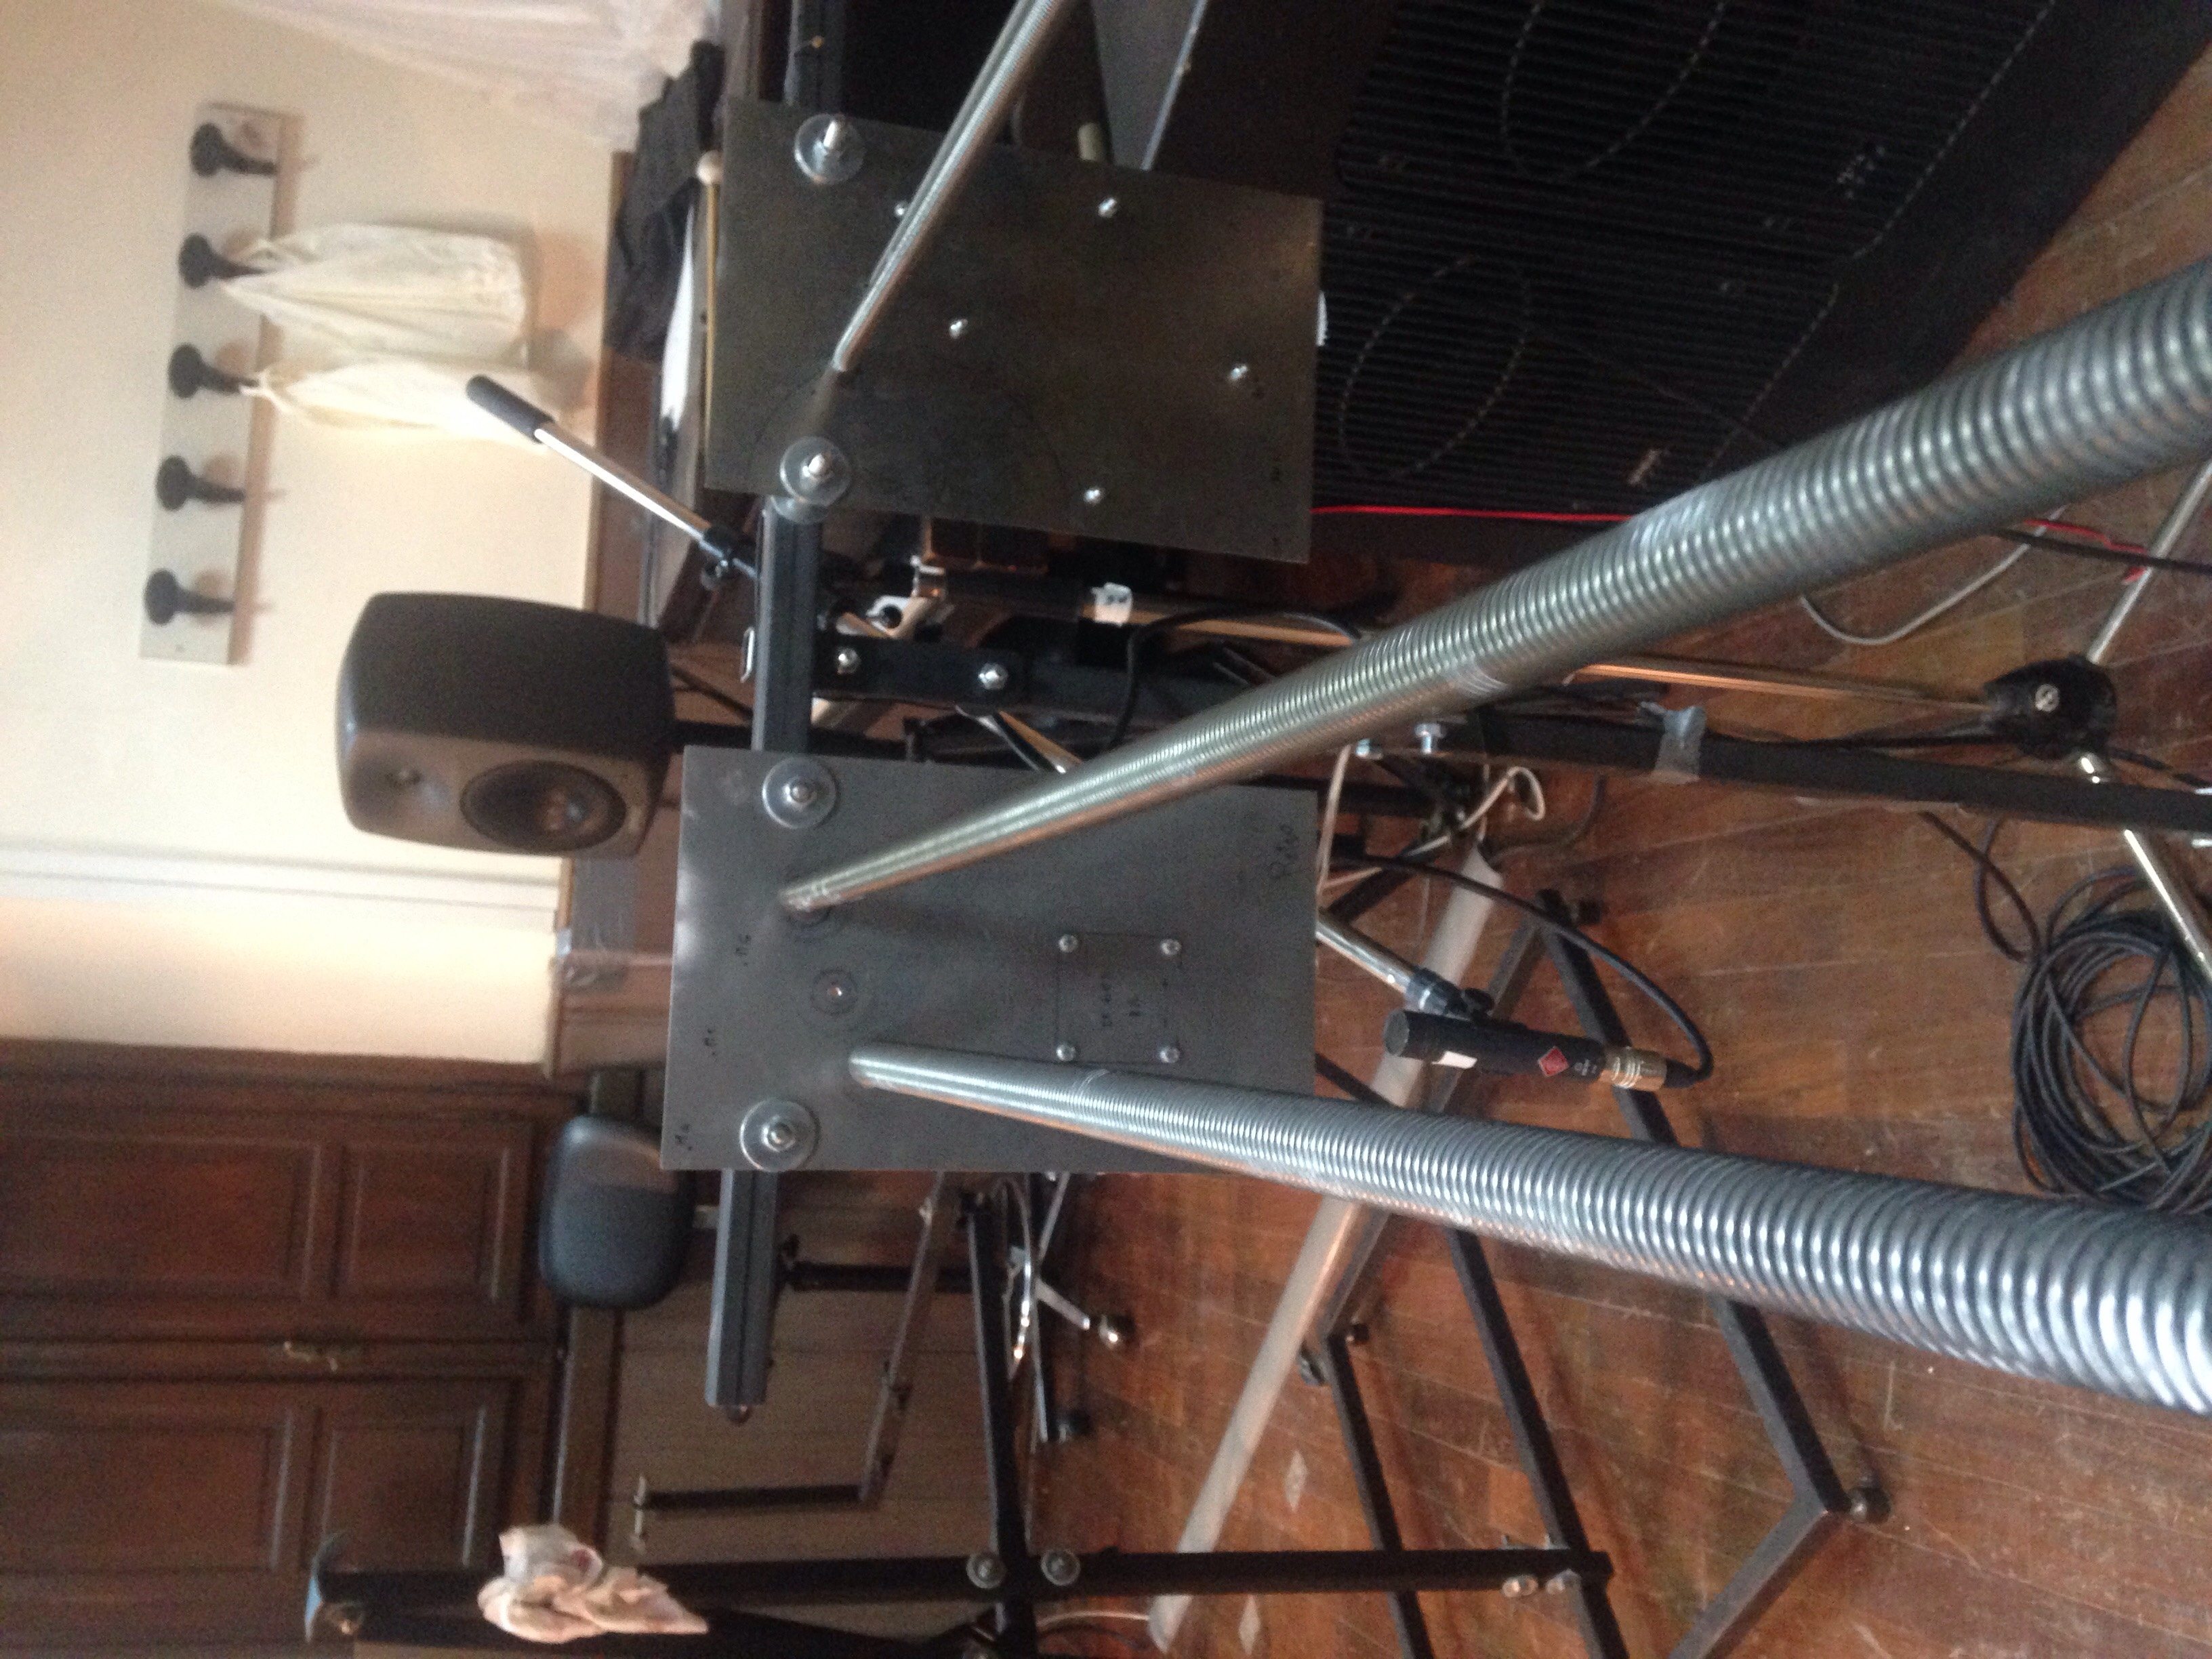
\epsfig{file=Spire2.jpg,width=8cm}}
\small{\caption{\textit{particolare}}}
\end{floatingfigure}
\textit{Sp.I.R.E.}, acronimo di \textit{Springs Installation Regulated \& Enhanced}, fa riferimento alla fisicità del materiale che compone lo strumento. Ogni molla (\textit{spring}) è formata da \textit{spire}. Il numero di tali spire rende possibile, a seconda del materiale col quale vengono eccitate, l'attivazione di armoniche e/o sub-armoniche. \\
\begin{floatingfigure}{10cm}
\mbox{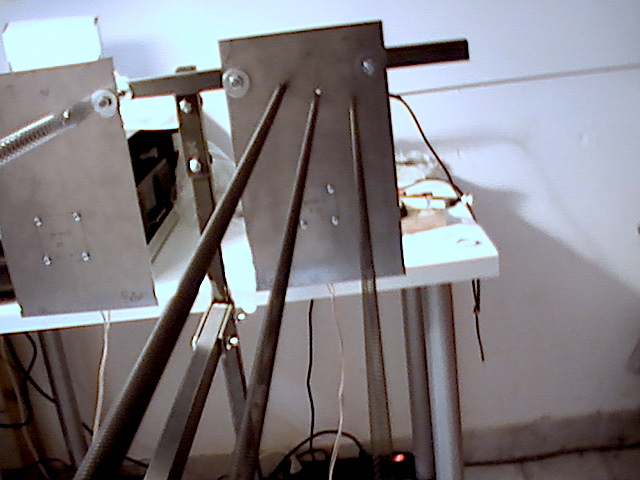
\epsfig{file=Prototipo02.jpg,width=8cm}}
\small{\caption{\textit{particolare}}}
\end{floatingfigure}
Questo esperimento è connesso allo studio di nuove identità formali relative alla natura dello strumento.  La ricerca è unita ad una realtà installativa dell'opera, che induce chi guarda e ascolta, a toccare la materia e ad incuriosirsi verso materiali come molle e placche di metallo, che sono stati creati per scopi lontani dall'utilizzo che ne viene fatto in questo determinato caso. \\
Spiego sinteticamente. Un basamento unisce due placche di metallo che montano su di esse, tre molle ciascuna, tese per la lunghezza paritaria di 80 centimetri. Durante la creazione di questo primo prototipo ho voluto utilizzarne solo cinque, sia per una questione di spazi che ti caratteristiche timbriche: alcune molle vicine di diametro andavano a provocare lo stessa timbrico. Ho perciò utilizzato in finale, cinque molle che per grandezza e risultante acustica erano diversificate maggiormente.\\ Il basamento è in ferro, le placche rettangolari, in acciaio armonico, le molle in ferro armonico. Nel primissimo prototipo una delle molle, la numero 4 era in acciaio inox, ma non avendo ottenuto i risultati timbrici sperati, ho deciso di cambiarla. Le molle sono disposte sulle placche in due sezioni a gradini, come se si andasse a suonare un violoncello, o un contrabbasso in posizione orizzontale. \\
Sp.i.r.e. è un progetto ambizioso che vuole, tra le altre cose, reinterpretare ed ampliare la visione di John Cage in Cartridge Music. Riuscire a rendere percepibili i suoni non udibili,  impercettibili, prodotti dallo strofinio delle molle e delle placche. \\
Ogni movimento sarà legato alle immagini di cordofoni classici, quindi durante la performance l'esecuzione avverrà con l'utilizzo di archetti per violoncello e contrabbasso. Da qui l'evoluzione del materiale in percussione o semplicemente in risonatore. \\ 
Come accennato, non disdegnerò in futuro una natura installativa e un'interattività dell'opera, ma soprattutto, per quanto interessante a livello timbrico fosse lo Sp.I.R.E. ancora non ero soddisfatto dei soli materiali sonori acustici. \\

\section{Intenzioni espressive}
\addcontentsline{toc}{section}{Intenzioni espressive (ideazione)}
\epigraph{\textbf{spirare} v. intr. e tr. [lat. spirare «soffiare»; respirare; emanare»]"}
{\textit{Enciclopedia Treccani}}

L'intenzione espressiva era perciò, la creazione di uno strumento che avesse in sé sia un reverbero a molle che un reverbero a piastra. Il risultato fu esaltante: le molle sfregate con dita o archetti generavano un ambiente sonoro che le piastre amplificavano e modificavano, generando una coda alla quale la placca univa la sua identità timbrica, dando vita a una sorta di \textit{convolutore naturale}. Sono cosciente dell'estremizzazione del significato di convolutore, anche perché, come sappiamo, il convolutore è la moltiplicazione delle sommatorie delle specifiche di due segnali: uno legato ad un ambiente di ripresa e uno legato ad uno strumento suonante. \\
\begin{floatingfigure}{10cm}
\mbox{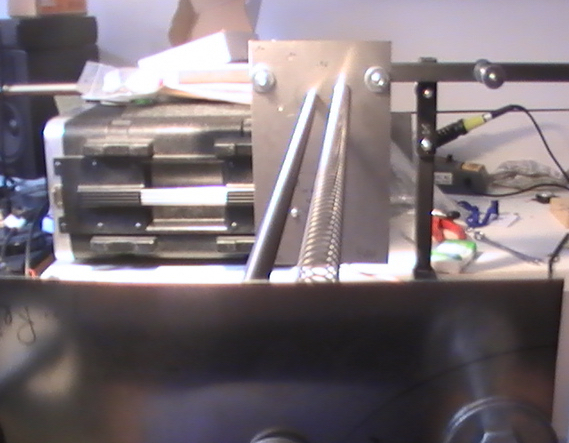
\epsfig{file=Prototipo3.jpg,width=9cm}}
\small{\caption{\textit{particolare}}}
\end{floatingfigure}
La svolta decisiva la ebbi durante il montaggio di Sp.I.R.E. perché decisi di aggiungere una variante elettroacustica: aggiunsi degli attuatori. Gli attuatori, diffusori a parete capaci di far interagire il materiale sul quale sono collocati con il suono diffuso, erano la variante finale per la messa a punto finale dell'opera.
Come scrive Silvia Lanzalone nel suo saggio sugli strumenti aumentati in \textit{Acustica}:
\begin{quotation}
\textit{La catena elettroacustica, nonostante il notevole perfezionamento tecnologico degli ultimi decenni verso l'accuratezza della riproduzione sonora, conferisce ancora al suono una trasformazione finale dovuta alla natura elettromeccanica dei suoi componenti, imponendovi dunque una deformazione che la rende decorrelata dal segnale che trasmette, nonché estranea ad esso dal punto di vista della sua identificazione percettiva nello spazio destinato alla sua diffusione}\footnote{Silvia Lanzalone \textit{Strumenti aumentati} in \textit{Acustica} UTET}.
\end{quotation} 

Spesso, quasi sempre, il suono elettronico risulta svincolato dal suono acustico. L'aggiunta e le prove sugli attuatori fissati sulle lastre è stato il passo successivo tenendo sempre a mente questo estratto. Agire come se si stesse "aumentando" uno strumento acustico è stato il pensiero principale, anche se stiamo parlando, nel caso di Sp.I.R.E., stiamo parlando di un oggetto sonoro più che di uno strumento. Ho provveduto, per le modifiche elettroacustiche, con gli stessi intenti con i quali si lavora per l'aumentazione di uno strumento di liuteria classica. Con la presenza degli attuatori, ho convogliato tutti i contributi elettronici (dall'elaborazione alla modulazione di frequenza) direttamente sullo strumento, così da evitare la divisione tra parte acustica ed elettronica e trasformando il mio oggetto sonoro in un vero e proprio strumento elettroacustico: possibilità di rilascio "acustico" del suono e quindi interazione tra elementi acustici ed elettronici. Si potrebbe quasi utilizzare l'appellativo di \textit{Iper-strumento}, perché è a tutti gli effetti uno strumento \textit{elettroacustico}, ha solo bisogno di una documentazione accurata e l'utilizzo in un certo numero di composizioni. \\
Ora che tutti i tratti somatici dello "strumento" erano delineati, potevo finalmente iniziare a pensare e scrivere una composizione ad hoc per Sp.I.R.E.. 

\section{Intenzioni estetiche}
\addcontentsline{toc}{section}{Intenzioni estetiche}
Il progetto va a rappresentare il legame con ciò che abbiamo attorno a noi, quello che siamo: tutt'uno con la metropoli e con l'ambiente che la circonda e va a formarla. \\
Questa è l'identità di Sp.i.r.e., finalmente si tocca con mano la parte nascosta della materia, il lato più nascosto di quello che vediamo attorno a noi. In unione ai suoni non udibili e all'invisibile, si scorge un richiamo verso una visione immaginifica che porta fino a dentro la nostra anatomia. Come se le spire della molla potessero essere ricondotte ai ripiegamenti dell'intestino; come se, all'eccitazione di una molla, si riconducesse la possibilità di produrre delle sub-armoniche e in qualche modo, di avvicinarsi alle vibrazioni interne dell'anatomia umana.\\
La meccanica, l'elettronica e i suoni analogici, rendono possibile la creazione di un mondo nuovo, e l'eccitazione delle molle mediante le placche di metallo fa sì che questa dimensione diventi parte della realtà umana. \\
Vengono a formarsi più dimensioni d'ascolto e più dimensioni tattili, causate dalle diverse risposte d'eccitazioni del materiale. A queste dimensioni d'ascolto si unisce la ripresa microfonica della performance, che sarà omnidirezionale e renderà possibile la riproduzione di tutto il panorama d'ascolto. Sp.i.r.e., anche nella sua identità installativa, respira ed emana il segnale elettroacustico in almeno due dimensioni d'ascolto:
\begin{enumerate} 
\item{\textit{Analogica}, la risposta del materiale ai suoni sintetici e al tocco umano}
\item{\textit{Elettrica ed elettronica}, che prende vita grazie ai suoni di sintesi diffusi dagli attuatori}
\end{enumerate}

L'insieme dei due fattori dava vita ad uno strumento che ha sia caratteristiche installative che performative. Una strana creature capace sia di suonare amplificata che acusticamente, ma che prende vita sopratutto grazie agli attuatori e al connubio fra placche e molle. La struttura è tutta \textit{suono}. Questo è comunque un primo esperimento e non mi fermerò prima di aver raggiunto determinati obbiettivi costruttivi, miglioramenti, che applicherò a breve sullo strumento. Come scrive Cage:
\begin{small}
\begin{quotation}
Decisi così di lavorare con qualunque strumento di produzione avessi incontrato e di tenere sempre un orecchio a terra, in cerca di un suono nuovo\footnote{John Cage, \textit{Confessioni di un compositore}}.
\end{quotation}
\end{small}
